

\tikzset{every picture/.style={line width=0.75pt}} %set default line width to 0.75pt        

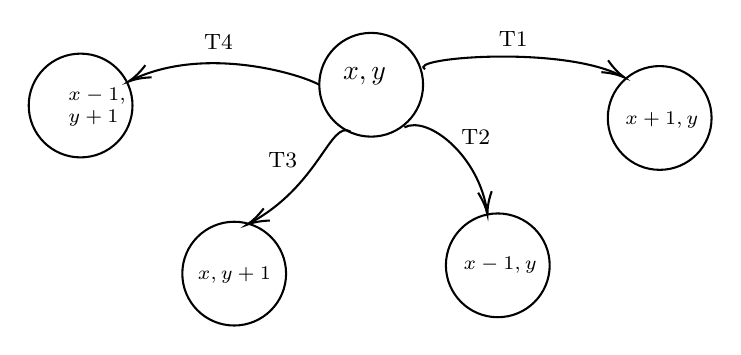
\begin{tikzpicture}[x=0.75pt,y=0.75pt,yscale=-1,xscale=1]
%uncomment if require: \path (0,300); %set diagram left start at 0, and has height of 300

%Shape: Circle [id:dp29754411522962854] 
\draw   (280,123) .. controls (280,109.19) and (291.19,98) .. (305,98) .. controls (318.81,98) and (330,109.19) .. (330,123) .. controls (330,136.81) and (318.81,148) .. (305,148) .. controls (291.19,148) and (280,136.81) .. (280,123) -- cycle ;
%Shape: Circle [id:dp49680162326801924] 
\draw   (419,139) .. controls (419,125.19) and (430.19,114) .. (444,114) .. controls (457.81,114) and (469,125.19) .. (469,139) .. controls (469,152.81) and (457.81,164) .. (444,164) .. controls (430.19,164) and (419,152.81) .. (419,139) -- cycle ;
%Shape: Circle [id:dp530060733071275] 
\draw   (140,133) .. controls (140,119.19) and (151.19,108) .. (165,108) .. controls (178.81,108) and (190,119.19) .. (190,133) .. controls (190,146.81) and (178.81,158) .. (165,158) .. controls (151.19,158) and (140,146.81) .. (140,133) -- cycle ;
%Shape: Circle [id:dp19184706057595724] 
\draw   (214,214) .. controls (214,200.19) and (225.19,189) .. (239,189) .. controls (252.81,189) and (264,200.19) .. (264,214) .. controls (264,227.81) and (252.81,239) .. (239,239) .. controls (225.19,239) and (214,227.81) .. (214,214) -- cycle ;
%Shape: Circle [id:dp701436760485959] 
\draw   (341,210) .. controls (341,196.19) and (352.19,185) .. (366,185) .. controls (379.81,185) and (391,196.19) .. (391,210) .. controls (391,223.81) and (379.81,235) .. (366,235) .. controls (352.19,235) and (341,223.81) .. (341,210) -- cycle ;
%Curve Lines [id:da8524812872961451] 
\draw    (280,123) .. controls (270.15,117.58) and (224.4,103.92) .. (189.58,120.71) ;
\draw [shift={(188,121.5)}, rotate = 332.78] [color={rgb, 255:red, 0; green, 0; blue, 0 }  ][line width=0.75]    (10.93,-3.29) .. controls (6.95,-1.4) and (3.31,-0.3) .. (0,0) .. controls (3.31,0.3) and (6.95,1.4) .. (10.93,3.29)   ;
%Curve Lines [id:da644127113209719] 
\draw    (295,145.5) .. controls (285.15,140.08) and (280.15,171.53) .. (246.55,189.68) ;
\draw [shift={(245,190.5)}, rotate = 332.78] [color={rgb, 255:red, 0; green, 0; blue, 0 }  ][line width=0.75]    (10.93,-3.29) .. controls (6.95,-1.4) and (3.31,-0.3) .. (0,0) .. controls (3.31,0.3) and (6.95,1.4) .. (10.93,3.29)   ;
%Curve Lines [id:da13651494423999866] 
\draw    (321,143.5) .. controls (332.76,137.62) and (357.01,157.67) .. (360.79,183.89) ;
\draw [shift={(361,185.5)}, rotate = 263.65999999999997] [color={rgb, 255:red, 0; green, 0; blue, 0 }  ][line width=0.75]    (10.93,-3.29) .. controls (6.95,-1.4) and (3.31,-0.3) .. (0,0) .. controls (3.31,0.3) and (6.95,1.4) .. (10.93,3.29)   ;
%Curve Lines [id:da9913763384642134] 
\draw    (331,115.5) .. controls (321.2,110.11) and (395.92,103.76) .. (425.26,118.57) ;
\draw [shift={(427,119.5)}, rotate = 209.74] [color={rgb, 255:red, 0; green, 0; blue, 0 }  ][line width=0.75]    (10.93,-3.29) .. controls (6.95,-1.4) and (3.31,-0.3) .. (0,0) .. controls (3.31,0.3) and (6.95,1.4) .. (10.93,3.29)   ;


% Text Node
\draw (290,113.4) node [anchor=north west][inner sep=0.75pt]    {$x,y$};
% Text Node
\draw (151,121.4) node [anchor=north west][inner sep=0.75pt]  [font=\scriptsize]  {$ \begin{array}{l}
x-1,\\
y+1
\end{array}$};
% Text Node
\draw (220,209.4) node [anchor=north west][inner sep=0.75pt]  [font=\scriptsize]  {$x,y+1$};
% Text Node
\draw (348,204.4) node [anchor=north west][inner sep=0.75pt]  [font=\scriptsize]  {$x-1,y$};
% Text Node
\draw (426,134.4) node [anchor=north west][inner sep=0.75pt]  [font=\scriptsize]  {$x+1,y$};
% Text Node
\draw (223,97) node [anchor=north west][inner sep=0.75pt]  [font=\footnotesize] [align=left] {T4};
% Text Node
\draw (365,96) node [anchor=north west][inner sep=0.75pt]  [font=\footnotesize] [align=left] {T1};
% Text Node
\draw (347,143) node [anchor=north west][inner sep=0.75pt]  [font=\footnotesize] [align=left] {T2};
% Text Node
\draw (254,154) node [anchor=north west][inner sep=0.75pt]  [font=\footnotesize] [align=left] {T3};


\end{tikzpicture}
